%% =====================================================================
% Capítulo: análisis y recuperación de Confidencial.pdf desde una imagen
% forense de Windows con carpeta Dropbox.
%
% Adaptado a partir de la estructura del capítulo del escenario USB y de
% la plantilla de informe pericial facilitada.
%
% IMPORTANTE:
% - Se han incorporado únicamente los datos aportados por el análisis.
% - Los campos marcados como TODO deben completarse con las comprobaciones
%   y evidencias que se obtengan durante el laboratorio.
% - No se afirma que el archivo se haya recuperado íntegramente ni que se
%   haya demostrado su eliminación desde la papelera: debe verificarse.
%
% Requiere los mismos comandos/paquetes que el documento principal:
%   \cod, booktabs, caption, listings (style=terminal), etc.
% =====================================================================

\subsection{Escenario 2: fuga mediante DropBox}
\label{cap:dropbox}

En este capítulo se documenta el segundo de los escenarios del enunciado: la fuga del fichero \cod{Confidencial.pdf} del \textit{Windows Server} 2008 mediante el servicio de almacenamiento online, Dropbox. En este caso tenemos una copia de la imagen del disco duro del dispositivo, desde donde se ha realizado la subida a Dropbox, pero que se supone que se ha eliminado del dispositivo. Nuestro trabajo en este caso consiste en realizar un análisis forense a partir de la imagen forense, en este caso la copia de la imagen del disco duro, comprobar si queda rastro del fichero recuperar el fichero, comprobar si se ha llegado a realizar una sincronización con la nube de Dropbox y mantener la cadena de custodia. 

\subsubsection{Planteamiento y alcance}
\begin{itemize}
	\item \textbf{Origen:} \cod{Confidencial.pdf} en el \textit{Windows Server}
	2008 configurado en la entrega anterior.
	\item \textbf{Soporte a analizar:} una copia de la imagen de disco duro que se nos entrega con el fichero ya eliminado
	\item \textbf{Entregable:} la copia de la imagen forense del disco duro, recuperación del fichero, cadena de custodia y conclusiones
	\item \textbf{Formato de la imagen:} la copia de la imagen forense del disco duro, se prepara en formato \textbf{RAW} (copia bit a bit, sin comprimir)
\end{itemize}

\subsection{Preparación y adquisición de la evidencia}

\subsubsection{Imagen forense analizada}

Se ha trabajado sobre la imagen \cod{W11.dd}, que se ha incorporado a
Autopsy para examinar su estructura de particiones y los sistemas de
archivos contenidos en ella. El fichero de imagen se utiliza como fuente
del análisis; las operaciones de extracción deben realizarse sobre copias
de trabajo, evitando modificar la evidencia original.

\begin{table}[H]
	\centering
	\small
	\renewcommand{\arraystretch}{1.3}
	\begin{tabular}{@{}p{0.34\textwidth}p{0.62\textwidth}@{}}
		\toprule
		\textbf{Característica} & \textbf{Valor} \\
		\midrule
		Nombre de la imagen & \cod{W11.dd} \\
		Formato & RAW / \cod{.dd} \\
		Volumen examinado & \cod{vol_vol6} \\
		Sistema de ficheros & NTFS \\
		Herramienta de análisis & Autopsy \\
		Herramienta complementaria & The Sleuth Kit (\cod{istat}) \\
		\bottomrule
	\end{tabular}
	\caption{Identificación de la fuente forense examinada.}
	\label{tab:dropbox-fuente}
\end{table}

% TODO: indicar el tamaño exacto de la imagen, su procedencia, fecha de
% adquisición y los hashes SHA-256/MD5 de la imagen, si se calcularon.
% TODO: añadir una captura de Autopsy donde se vea la imagen y el volumen.

% ---------------------------------------------------------------------
\subsection{Localización del fichero en Autopsy}

Durante el examen del volumen \cod{vol_vol6}, Autopsy mostró una entrada
asociada al nombre \cod{Confidencial.pdf}, situada en la ruta lógica
\cod{Users/Pepe/Dropbox/Confidencial.pdf}. La ficha de metadatos presenta
un tamaño de 103 bytes y un tipo MIME identificado como
\cod{text/plain}.

Los campos de asignación del nombre y de los metadatos aparecen como
\textit{Unallocated}. Por tanto, la entrada se encuentra marcada como no
asignada según la interpretación que presenta Autopsy. La existencia de
metadatos consultables no implica necesariamente que todos los bloques
del contenido continúen disponibles.

\begin{table}[H]
	\centering
	\small
	\renewcommand{\arraystretch}{1.25}
	\begin{tabular}{@{}p{0.37\textwidth}p{0.59\textwidth}@{}}
		\toprule
		\textbf{Campo de Autopsy} & \textbf{Valor observado} \\
		\midrule
		Name & \cod{/W11.dd/vol_vol6/Users/Pepe/Dropbox/Confidencial.pdf} \\
		Type & File System \\
		MIME Type & \cod{text/plain} \\
		Size & 103 bytes \\
		File Name Allocation & Unallocated \\
		Metadata Allocation & Unallocated \\
		Modified & 2026-11-19 19:15:29 CET \\
		Accessed & 2026-11-19 19:15:22 CET \\
		Created & 2026-11-11 21:35:24 CET \\
		Changed & 2026-11-19 19:15:29 CET \\
		MD5 & 4c9283480e5692410e177df58323e732 \\
		SHA-256 & f3ff86db9d526b85bab2afaf03722c321392f8b8dcae558d583704d713ef3fa7 \\
		Internal ID & 615530 \\
		\bottomrule
	\end{tabular}
	\caption{Metadatos del fichero mostrados por Autopsy.}
	\label{tab:dropbox-autopsy}
\end{table}

\begin{figure}[H]
	\centering
	% TODO: sustituir por la captura real de Autopsy.
	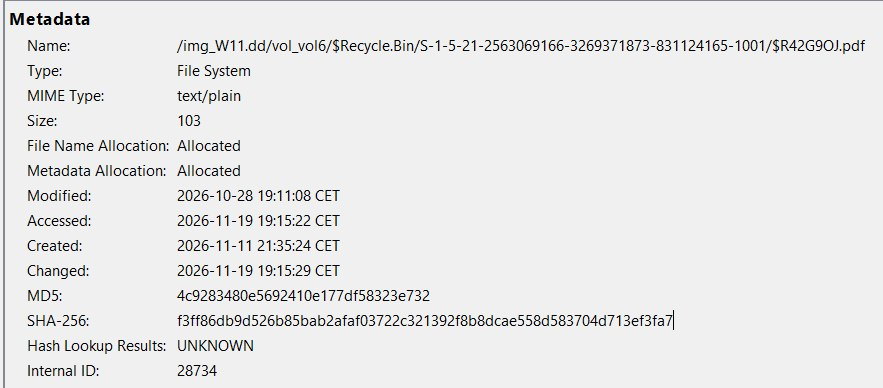
\includegraphics[width=0.9\textwidth]{Recursos/dropbox_autopsy_metadatos.jpg}
	\caption{Metadatos del fichero \cod{Confidencial.pdf} en Autopsy.}
	\label{fig:dropbox-autopsy}
\end{figure}

\subsection{Examen de la entrada MFT mediante The Sleuth Kit}

Con el objetivo de ampliar la información obtenida mediante Autopsy,
se ha examinado la entrada MFT asociada al fichero
\cod{Confidencial.pdf} utilizando la herramienta \cod{istat} de
The Sleuth Kit.

El registro identificado corresponde a la entrada MFT 188015,
con número de secuencia 5. El análisis de sus atributos permite
examinar la identificación del fichero, sus marcas temporales,
los flujos de datos asociados y su relación con los elementos
localizados en la papelera de reciclaje de Windows.

\subsubsection{Identificación del registro}

La salida de \cod{istat} proporciona los siguientes datos
de identificación:

\begin{table}[H]
	\centering
	\small
	\renewcommand{\arraystretch}{1.25}
	\begin{tabular}{@{}p{0.40\textwidth}p{0.56\textwidth}@{}}
		\toprule
		\textbf{Campo} & \textbf{Valor observado} \\
		\midrule
		MFT Entry & 188015 \\
		Sequence & 5 \\
		\cod{\$LogFile} Sequence Number & 1880141102 \\
		Estado indicado por \cod{istat} & Allocated File \\
		Links & 2 \\
		Parent MFT Entry & 159329 \\
		Parent Sequence & 4 \\
		\cod{\$FILE\_NAME} & \cod{\$R42G9OJ.pdf} \\
		Allocated Size & 104 bytes \\
		Actual Size & 103 bytes \\
		\bottomrule
	\end{tabular}
	\caption{Datos de identificación de la entrada MFT 188015.}
	\label{tab:dropbox-mft-identificacion}
\end{table}

El atributo \cod{\$FILE\_NAME} muestra el nombre
\cod{\$R42G9OJ.pdf}, mientras que Autopsy presenta la ruta lógica
terminada en \cod{Confidencial.pdf}. Esta diferencia es compatible
con la nomenclatura utilizada por la papelera de reciclaje de Windows.

La relación entre ambos nombres se ha contrastado mediante los
archivos de metadatos \cod{\$I} localizados durante el análisis.
Estos contienen la ruta original:

\begin{lstlisting}[style=terminal,breaklines=true]
	C:\Users\Pepe\Dropbox\Confidencial.pdf
\end{lstlisting}

Asimismo, los metadatos indican un tamaño original de 103 bytes.
La ubicación de los elementos dentro de la estructura
\cod{\$Recycle.Bin}, junto con la correspondencia entre los nombres
\cod{\$I} y \cod{\$R}, permite relacionar el registro examinado
con el elemento eliminado.

\subsubsection{Atributo \cod{\$STANDARD\_INFORMATION}}

El atributo \cod{\$STANDARD\_INFORMATION} contiene las marcas
temporales y otros datos asociados al registro. Según la salida
de \cod{istat}, se han obtenido los siguientes valores:

\begin{table}[H]
	\centering
	\small
	\renewcommand{\arraystretch}{1.25}
	\begin{tabular}{@{}p{0.39\textwidth}p{0.57\textwidth}@{}}
		\toprule
		\textbf{Campo} & \textbf{Valor observado} \\
		\midrule
		Flags & Archive \\
		Owner ID & 0 \\
		Security ID & 3104 \\
		SID asociado &
		\cod{S-1-5-21-2563069166-3269371873-831124165-1001} \\
		Last User Journal Update Sequence Number & 388781040 \\
		Created & 2026-11-11 21:35:24.879494100 (CET) \\
		File Modified & 2026-10-28 20:11:08.119424400 (CET) \\
		MFT Modified & 2026-11-19 19:15:29.239077300 (CET) \\
		Accessed & 2026-11-19 19:15:22.259298700 (CET) \\
		\bottomrule
	\end{tabular}
	\caption{Valores del atributo
		\cod{\$STANDARD\_INFORMATION}.}
	\label{tab:dropbox-standard-information}
\end{table}

La fecha de modificación del contenido registrada en la entrada
MFT es anterior a la fecha de creación del registro. Por otra
parte, la modificación de la entrada MFT se produjo el
19/11/2026 a las 19:15:29, mientras que el último acceso
registrado corresponde a las 19:15:22 del mismo día.

Estas marcas temporales representan campos distintos y no deben
interpretarse como prueba aislada de una acción concreta.
La diferencia entre la fecha de modificación del contenido
y la fecha de creación de la entrada puede ser compatible
con una copia, descarga, restauración u otra operación
sobre el fichero.

\subsubsection{Atributo \cod{\$FILE\_NAME}}

El atributo \cod{\$FILE\_NAME} recoge el nombre
\cod{\$R42G9OJ.pdf}, la referencia a la entrada MFT padre
159329, con número de secuencia 4, y los tamaños asignado
y real de 104 y 103 bytes, respectivamente.

La nomenclatura \cod{\$R...} es relevante porque Windows utiliza
nombres con prefijos \cod{\$I} y \cod{\$R} para almacenar,
respectivamente, los metadatos y el contenido de los elementos
eliminados de la papelera de reciclaje.

En este caso, la correspondencia con los archivos de metadatos
\cod{\$I} permite asociar el registro con el fichero original
\cod{Confidencial.pdf}.

\subsubsection{Atributo \cod{\$OBJECT\_ID}}

La entrada MFT contiene también un atributo
\cod{\$OBJECT\_ID}, cuyo identificador es:

\begin{lstlisting}[style=terminal,breaklines=true]
	13b844df-e442-11f1-afe0-080027541882
\end{lstlisting}

Este identificador se conserva como dato técnico del registro
examinado. Por sí solo no permite identificar al usuario que
realizó una operación ni establecer el momento exacto
de eliminación del fichero.

\subsubsection{Atributos de datos}

La salida de \cod{istat} identifica dos atributos de datos
asociados a la entrada MFT:

\begin{itemize}
	\item \cod{\$DATA} (128-1), sin nombre, residente,
	con un tamaño de 103 bytes.
	\item \cod{\$DATA} (128-7), denominado
	\cod{com.dropbox.attrs}, residente,
	con un tamaño de 26 bytes.
\end{itemize}

El primer atributo corresponde al flujo de datos principal
del fichero. El segundo es un flujo de datos alternativo
con nombre asociado a Dropbox.

La presencia de \cod{com.dropbox.attrs} acredita que la entrada
MFT contiene un atributo adicional con ese nombre. Este dato
es relevante para contextualizar la relación del fichero
con Dropbox, aunque no demuestra por sí solo que el contenido
se haya sincronizado correctamente con el servicio remoto.

\subsubsection{Correlación con los archivos de la papelera}

Durante el análisis se localizaron dos archivos de metadatos
de la papelera, denominados \cod{\$IDRIES9.pdf} y
\cod{\$I42G9OJ.pdf}. Ambos hacen referencia a la ruta original \\
\cod{C:/Users/Pepe/Dropbox/Confidencial.pdf}
y a un tamaño original de 103 bytes.

Las marcas temporales contenidas en ambos archivos reflejan
dos eventos de eliminación separados por aproximadamente
30 segundos. La existencia de ambos registros debe documentarse
sin atribuir una causa concreta a la duplicidad, ya que no se
ha establecido qué operación originó cada evento.

La correspondencia entre los archivos de metadatos
\cod{\$I}, el archivo de contenido \cod{\$R42G9OJ.pdf}
y la ruta original permite relacionar la entrada MFT
examinada con el fichero \cod{Confidencial.pdf} localizado
en la carpeta de Dropbox.

\begin{figure}[H]
	\centering
	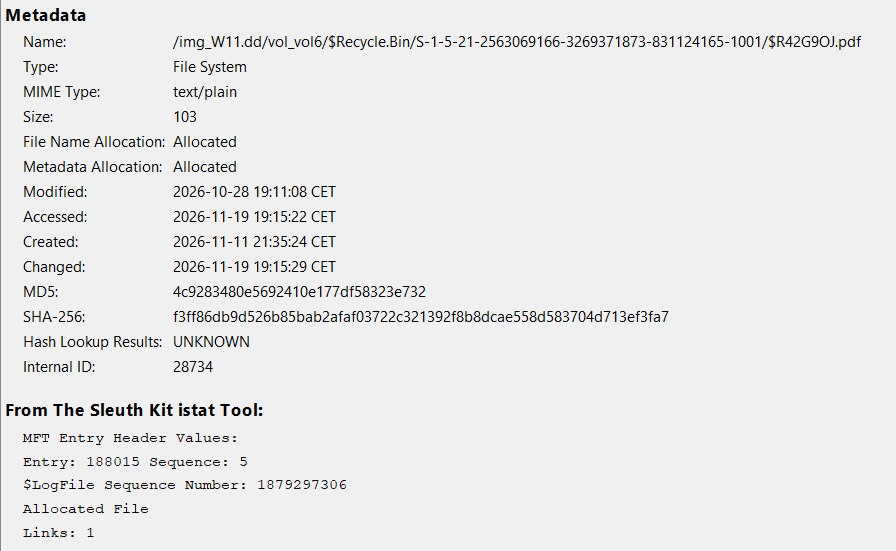
\includegraphics[width=0.95\textwidth]{Recursos/dropbox_istat.jpg}
	\caption{Examen de la entrada MFT mediante The Sleuth Kit.}
	\label{fig:dropbox-istat}
\end{figure}


% ---------------------------------------------------------------------
\subsection{Examen de artefactos locales de Dropbox}
\label{sec:dropbox-artefactos}

Durante el análisis recursivo del volumen NTFS mediante The Sleuth Kit
se localizaron diversos artefactos pertenecientes a la instalación de
Dropbox. Los archivos se encuentran principalmente bajo la ruta:

\begin{lstlisting}[style=terminal,breaklines=true]
	Users/Pepe/AppData/Local/Packages/
	DropboxInc.Dropbox_xbfy0k16fey96/LocalCache/Local/Dropbox/
\end{lstlisting}

La ubicación corresponde a una estructura de almacenamiento de la
aplicación Dropbox instalada en Windows. Esta ruta explica que no se
haya localizado necesariamente la configuración en el directorio
tradicional \cod{AppData/Local/Dropbox}.

Entre los artefactos identificados se encuentran los siguientes:

\begin{table}[H]
	\centering
	\small
	\renewcommand{\arraystretch}{1.25}
	\begin{tabular}{@{}p{0.43\textwidth}p{0.51\textwidth}@{}}
		\toprule
		\textbf{Artefacto} & \textbf{Ubicación o función a investigar} \\
		\midrule
		\cod{info.json} & Configuración de la carpeta local de Dropbox \\
		\cod{host.db} & Información local asociada a la ruta de Dropbox \\
		\cod{host.dbx} & Artefacto de configuración de Dropbox \\
		\cod{sync_history.db} & Historial local de eventos \\
		\cod{nucleus.sqlite3} & Base de datos del sistema de sincronización \\
		\cod{nucleus.sqlite3-wal} & Registro WAL asociado a la base anterior \\
		\cod{apex.sqlite3} & Base de datos interna de Dropbox \\
		\cod{apex.sqlite3-wal} & Registro WAL asociado a la base anterior \\
		\cod{config.dbx} & Archivo de configuración de la instancia \\
		\cod{unlink.db} & Artefacto relacionado con la instancia de Dropbox \\
		\bottomrule
	\end{tabular}
	\caption{Artefactos locales de Dropbox identificados en el volumen.}
	\label{tab:dropbox-artefactos}
\end{table}

El archivo \cod{info.json} contiene una configuración personal de Dropbox
y especifica la ruta local:

\begin{lstlisting}[style=terminal,breaklines=true]
	C:\Users\Pepe\Dropbox
\end{lstlisting}

El contenido también indica que la configuración no corresponde a una
cuenta de equipo y que el tipo de suscripción registrado es \cod{Basic}.
El archivo \cod{host.db} contiene igualmente la ruta local codificada
en Base64, lo que proporciona una segunda referencia a la carpeta
utilizada por Dropbox.

La presencia de estos artefactos permite acreditar la existencia de
información de configuración local de Dropbox en el sistema analizado.
No demuestra por sí sola que un archivo concreto se haya subido
correctamente a los servidores del servicio.


% ---------------------------------------------------------------------
\subsection{Análisis del historial de sincronización}
\label{sec:dropbox-sync-history}

Se extrajo y examinó la base de datos \cod{sync_history.db}, localizada
en el directorio de sincronización de la instancia de Dropbox. El archivo
corresponde a la entrada MFT 166315, secuencia 6, y presenta un tamaño
de 8192 bytes.

La base de datos SQLite contiene una tabla denominada
\cod{sync\_history}. Durante su análisis se identificó un registro que
hace referencia expresamente al fichero investigado.

\begin{table}[H]
	\centering
	\small
	\renewcommand{\arraystretch}{1.25}
	\begin{tabular}{@{}p{0.37\textwidth}p{0.57\textwidth}@{}}
		\toprule
		\textbf{Campo} & \textbf{Valor observado} \\
		\midrule
		\cod{event\_type} & \cod{file} \\
		\cod{file\_event\_type} & \cod{delete} \\
		\cod{direction} & \cod{upload} \\
		\cod{file\_id} & \cod{s7HUet7Mk4EAAAAAAAAABQ} \\
		\cod{local\_path} &
		\cod{C:/Users/Pepe/Dropbox/Confidencial.pdf} \\
		\cod{server\_path} & \cod{NULL} \\
		\cod{other\_user} & \cod{0} \\
		\cod{timestamp} & \cod{1795112171} \\
		\bottomrule
	\end{tabular}
	\caption{Registro de \cod{sync\_history.db} asociado a
		\cod{Confidencial.pdf}.}
	\label{tab:dropbox-sync-history}
\end{table}

El valor del campo \cod{timestamp} corresponde al 19 de noviembre de
2026, a las 19:16:11, en hora peninsular española.

La coincidencia de la ruta local con el fichero investigado constituye
una referencia directa a \cod{Confidencial.pdf} dentro del historial
local de Dropbox. Asimismo, el campo \cod{direction} presenta el valor
\cod{upload}, asociado a una dirección de subida.

No obstante, el campo \cod{file\_event\_type} presenta el valor
\cod{delete} y el campo \cod{server\_path} aparece como
\cod{NULL}. Por tanto, el registro debe interpretarse como un evento
de eliminación relacionado con una dirección de subida, sin que permita
confirmar de forma concluyente que el fichero permaneciese almacenado en la nube.

La base de datos superó la comprobación de integridad de SQLite,
obteniéndose el resultado \cod{ok}.


% ---------------------------------------------------------------------
\subsection{Correlación temporal de los artefactos}
\label{sec:dropbox-cronologia}

Se han comparado las marcas temporales de los archivos de configuración
de Dropbox, las entradas de la papelera y el registro de actividad
local. Los tiempos se expresan en hora peninsular española (CET).

\begin{table}[H]
	\centering
	\small
	\renewcommand{\arraystretch}{1.25}
	\begin{tabular}{@{}p{0.28\textwidth}p{0.30\textwidth}p{0.36\textwidth}@{}}
		\toprule
		\textbf{Fecha y hora} & \textbf{Artefacto} & \textbf{Evento observado} \\
		\midrule
		19/11/2026 19:13:49 &
		\cod{nucleus.sqlite3} &
		Creación de la base de datos principal \\
		
		19/11/2026 19:13:54--19:13:55 &
		\cod{info.json}, \cod{host.dbx} &
		Creación de archivos de configuración \\
		
		19/11/2026 19:14:17 &
		\cod{host.dbx} &
		Modificación del archivo de configuración \\
		
		19/11/2026 19:14:58 &
		\cod{\$IDRIES9.pdf} &
		Primer registro de eliminación del archivo \\
		
		19/11/2026 19:15:29 &
		\cod{\$I42G9OJ.pdf} &
		Segundo registro de eliminación del archivo \\
		
		19/11/2026 19:16:11 &
		\cod{sync\_history.db} &
		Modificación de la base de datos y timestamp del evento registrado \\
		\bottomrule
	\end{tabular}
	\caption{Cronología de los artefactos relacionados con Dropbox y
		\cod{Confidencial.pdf}.}
	\label{tab:dropbox-cronologia}
\end{table}

La proximidad temporal entre la actividad de los archivos de configuración,
los registros de eliminación y el evento almacenado en
\cod{sync\_history.db} resulta relevante para la investigación.

La cronología se utiliza como elemento de contextualización y debe
valorarse conjuntamente con el contenido de los artefactos.

\subsection{Conclusiones del análisis}
\label{sec:dropbox-conclusiones}

El análisis de la imagen forense ha permitido localizar artefactos
asociados al fichero \cod{Confidencial.pdf}, cuya ruta lógica se sitúa
en \cod{Users/Pepe/Dropbox/Confidencial.pdf}. El fichero presenta un
tamaño de 103 bytes.

La entrada MFT 188015, secuencia 5, contiene un atributo de datos
principal residente de 103 bytes y un flujo alternativo denominado
\cod{com.dropbox.attrs}, de 26 bytes. Asimismo, se localizaron dos
archivos de metadatos de la papelera que hacen referencia a la ruta
original y al tamaño del fichero.

En el sistema se identificaron archivos de configuración y bases de
datos locales de Dropbox. El contenido de \cod{info.json} y
\cod{host.db} vincula la configuración local con la carpeta
\cod{C:/Users/Pepe/Dropbox}.

El hallazgo más relevante es el registro de
\cod{sync\_history.db}, que menciona expresamente la ruta de
\cod{Confidencial.pdf}, contiene un identificador de archivo y presenta
el valor \cod{upload} en el campo \cod{direction}. Este registro
constituye un indicio significativo de una operación de subida
relacionada con el fichero.

La proximidad temporal entre el registro de actividad de Dropbox y
los eventos de eliminación es muestra de que el fichero
estuvo involucrado en actividad de sincronización. Por ello, los resultados permiten
confirmar de forma concluyente que el archivo permaneciese almacenado en los servidores de Dropbox.

En consecuencia, con los artefactos disponibles puede confirmarse la
sospecha fundada de una operación de subida asociada a
\cod{Confidencial.pdf}.

\subsection{Evidencias}

Para la elaboración de este apartado se han utilizado los resultados
obtenidos durante el examen de la imagen forense \cod{W11.dd} mediante
Autopsy y The Sleuth Kit.

\begin{enumerate}
	\item Imagen forense original:
	\cod{W11.dd} \\
	SHA256: 13A197F9BA22B95CAD728E14DFBEA44A4A09C16419352EBA6EE76D506D40D98B
	\item Registro MFT examinado:
	entrada 188015, secuencia 5, correspondiente al registro que
	contiene el nombre \cod{\$R42G9OJ.pdf}.	
\end{enumerate}